%****************************** Preámbulo ******************************%
\documentclass[letterpaper, 12pt]{article}

% <<< BEGIN idioma y codificación

% Idioma de trabajo: español, "table" -> "tabla" y punto decimal en fórmulas (sin la opción sería coma).
\usepackage[spanish, es-tabla, es-nodecimaldot]{babel}

% Acentos, ñ y separación silábica correcta de palabras acentuadas.
\usepackage[utf8]{inputenc}
\usepackage[T1]{fontenc}
\usepackage{lmodern}

% >>> END

% <<< BEGIN paquetes y macros

% Imágenes y ubicación fija de figuras con \begin{figure}[H].
\usepackage{graphicx}
\usepackage{float}
\graphicspath{{images/}}

% Notación (derivadas, vectores, brakets, unidades) y entornos matemáticos.
\usepackage{physics, amsmath, amssymb}

% Tablas con líneas horizontales limpias (\toprule, \midrule, \bottomrule).
\usepackage{booktabs}

% Gráficos con el lenguaje nativo de LaTeX.
\usepackage{tikz}
\usetikzlibrary{fit, backgrounds, arrows.meta, positioning, babel}

% Colores para gráficas y diagramas TikZ (los mismos del template de Beamer).
% Los colores UNAM (UNAMDarkBlue, UNAMLightBlue, UNAMGold) vienen de unampaper.sty.
\definecolor{myblue}{RGB}{30,100,180}
\definecolor{myred}{RGB}{180,30,30}
\definecolor{mygreen}{RGB}{20,140,60}
\definecolor{mypurple}{RGB}{120,30,160}
\definecolor{myorange}{RGB}{220,120,0}

% Listas con formato configurable (mejor que enumerate a secas).
\usepackage{enumitem}

% Texto a dos columnas: \begin{multicols}{2} ... \end{multicols}.
\usepackage{multicol}
\setlength\columnsep{20pt}

% Fórmulas más grandes dentro del texto (útil en ejercicios resueltos).
\usepackage{relsize}
\newcommand{\mlr}[1]{\mbox{$\mathlarger{#1}$}}

% Unidades: 9.8\un{m/s$^2$}.
\newcommand{\un}[1]{\mbox{ #1}}

% Citas como superíndice.
\newcommand{\upcite}[1]{\mbox{$^\text{\cite{#1}}$}}

% Árbol de directorios.
\usepackage{dirtree}

% Macros del proyecto.
\newcommand{\hMpc}{\ensuremath{h^{-1}\,\mathrm{Mpc}}}
\newcommand{\DD}{\mathrm{DD}}
\newcommand{\DR}{\mathrm{DR}}
\newcommand{\RR}{\mathrm{RR}}
\newcommand{\LCDM}{\Lambda\mathrm{CDM}}

% >>> END

% <<< BEGIN estilo UNAM

% Márgenes, título, índice, PromptBlock y enlaces (colores UNAM solo en enlaces).
% Va al final del preámbulo porque carga hyperref.
\usepackage{unampaper}

% >>> END

% <<< BEGIN metadatos

\title{Covarianza de los estimadores de la función de correlación en un modelo de dilución de materia oscura}
\author{Jair Ferrara Andrade}
% \date{Diciembre 2026}   % opcional

% >>> END

%****************************** Documento ******************************%
\begin{document}

    % Numeración romana desde la portada.
    \pagenumbering{Roman}

    \maketitle

    \begin{abstract}
        Se presenta un estudio de la covarianza de cuatro estimadores de la función de correlación de dos puntos, $\xi(r)$, en un modelo de dilución de materia oscura: Peebles--Hauser, Davis--Peebles, Hamilton y Landy--Szalay. En este modelo, una fuente en la ecuación de continuidad diluye las perturbaciones de materia sin modificar la expansión $\LCDM$ del fondo, de modo que, a orden lineal, el espectro de potencias solo cambia de amplitud: $P_{\rm dil} = 0.80\,P_{\LCDM}$ en $z = 0.5$. Para medir la covarianza se generan $5\times10^4$ realizaciones de campos gaussianos por modelo en una caja periódica de $1\,h^{-3}\,\mathrm{Gpc}^3$, muestreadas con $\bar n = 5\times10^{-5}\,h^{3}\,\mathrm{Mpc}^{-3}$, y en cada una se miden los cuatro estimadores. Los promedios reproducen el $\xi(r)$ teórico, incluido el pico BAO, salvo un sesgo que aparece por usar el mismo catálogo aleatorio en todas las realizaciones. La varianza con dilución resulta ser entre $0.953$ y $0.971$ veces la de $\LCDM$, según el estimador y el tamaño del catálogo aleatorio, muy lejos del $0.64$ que se esperaría si solo hubiera varianza cósmica, porque con esta densidad de puntos domina el ruido de Poisson. Aunque la señal cambia en un 20\%, la covarianza casi no distingue entre los dos modelos. Por último, como en la caja no hay bordes, Landy--Szalay y Hamilton resultan ser los estimadores con mayor varianza, y los cocientes entre estimadores siguen una estimación de Poisson sencilla.
    \end{abstract}

    \unamindice

    %=====================================================================%
    \section{Modelo de dilución}\label{sec:modelo}
    %=====================================================================%

        \subsection{Motivación}

            La motivación de este trabajo parte de una tensión pequeña, pero persistente: en $\LCDM$ plano, las mediciones de oscilaciones acústicas de bariones (BAO) de DESI DR2 prefieren una densidad de materia $\Omega_m$ menor que la que se infiere del fondo cósmico de microondas (CMB) \cite{desi_dr2, planck2018}. En el plano $\Omega_m$--$hr_d$, la diferencia va de $2.0$ a $3.7\sigma$, dependiendo del conjunto de datos del CMB que se use \cite{camphuis}. Esto no es evidencia de que exista un intercambio de energía en el sector oscuro, pero sí abre la pregunta de si parte de lo que se le atribuye a la energía oscura podría venir, en realidad, de un cambio en la materia \cite{chen_loeb, aviles_ferrara}.

            Los modelos con interacciones en el sector oscuro no solo modifican la expansión, también modifican el crecimiento de las perturbaciones. Por ejemplo, pueden producir un $w<-1$ aparente junto con un $S_8$ menor \cite{khoury2025, khoury2026} o cambiar las correcciones no lineales del espectro de potencias \cite{silva}. Esto es importante porque dos modelos con la misma historia de expansión pueden tener un agrupamiento distinto y, por lo tanto, son las perturbaciones las que permiten distinguirlos \cite{aviles_ferrara}.

            El punto de partida es el modelo de dilución de materia oscura de Avilés y Ferrara \cite{aviles_ferrara}. En esta sección se resume la parte del modelo que se usa aquí, es decir, el orden lineal en espacio real hasta llegar al espectro de potencias $P_{\rm dil}(k)$. Las predicciones de la Sección~\ref{sec:predicciones} y todo lo que sigue después corresponden al trabajo desarrollado en este proyecto.

        \subsection{Continuidad con una fuente}

            La idea del modelo es sencilla: si la materia oscura puede cederle energía a otra componente, entonces su ecuación de continuidad ya no está igualada a cero, sino a una fuente $S(\vb{x},t)$. El promedio espacial de esta fuente, $\bar S(t) = \expval{S}_{\vb{x}}$, es la que siente el fondo:

            \begin{equation}\label{eq:continuidad}
                \dot\rho + 3H\rho + \frac{1}{a}\nabla\cdot(\rho\,\vb{v}) = S, \qquad
                \dot{\bar\rho} + 3H\bar\rho = \bar S.
            \end{equation}

            En estas expresiones, $\rho$ es la densidad de materia, $\bar\rho$ la densidad de fondo y $\vb{v}$ la velocidad peculiar. Al restar la ecuación del fondo, el contraste de densidad $\delta = \rho/\bar\rho - 1$ satisface

            \begin{equation}\label{eq:contraste}
                \dot\delta + \frac{1}{a}\nabla\cdot\qty[(1+\delta)\,\vb{v}] = \frac{S - (1+\delta)\bar S}{\bar\rho},
            \end{equation}

            mientras que las ecuaciones de Euler y de Poisson se quedan como siempre:

            \begin{equation}\label{eq:euler_poisson}
                \dot{\vb{v}} + H\vb{v} + \frac{1}{a}(\vb{v}\cdot\nabla)\vb{v} = -\frac{1}{a}\nabla\Phi, \qquad
                \nabla^2\Phi = \frac{3}{2}\,\Omega_m H^2 a^2\,\delta.
            \end{equation}

            Todo depende entonces de cómo se escoja la fuente. Si $S = \Gamma\rho$, con $\Gamma$ una tasa de interacción como en los modelos de energía oscura interactuante, entonces $\bar S = \Gamma\bar\rho$ y el lado derecho de la ecuación \eqref{eq:contraste} se anula: la fuente cambia el fondo, pero el contraste evoluciona igual que siempre. En cambio, si $S = -gH\bar\rho\,\delta$ con $\bar S = 0$, el lado derecho es $-gH\delta$: el fondo sigue siendo $\LCDM$ y lo que se diluye son las perturbaciones, con una tasa $gH$. Una forma de verlo es pensar en una sobredensidad. Con la primera fuente, la región densa y su entorno pierden materia en la misma proporción y el contraste no cambia; con la segunda, la región densa pierde materia mientras que el fondo no, así que la sobredensidad se aplana.

            El modelo de dilución usa la segunda opción \cite{aviles_ferrara}. Como $g(t)$ es uniforme en el espacio, no introduce ninguna escala nueva, y tampoco se supone ningún mecanismo microscópico para la componente que recibe la materia. En la formulación lagrangiana de \cite{aviles_ferrara}, esto se traduce en que la masa que transporta cada elemento de fluido deja de conservarse, pero aquí solo hace falta el resultado a orden lineal.

        \subsection{\texorpdfstring{\emph{Toy model}}{Toy model}}

            Para la tasa de dilución se usa el \emph{toy model} de \cite{aviles_ferrara}:

            \begin{equation}\label{eq:toy}
                g(z) = \frac{g_0}{2}\qty[1 - \tanh\qty(\frac{z - z_t}{\Delta z})],
            \end{equation}

            con $g_0 = 0.2$, $z_t = 2$ y $\Delta z = 0.2$, sobre un fondo $\LCDM$ plano con $\Omega_{m0} = 0.3$. La tangente hiperbólica funciona como un interruptor: para $z \gg z_t$ se tiene $g \to 0$ y se recupera $\LCDM$, mientras que para $z \ll z_t$ se tiene $g \to g_0$ y la dilución está activa (véase la Figura~\ref{fig:crecimiento}). El ancho $\Delta z$ controla qué tan rápido se prende. Al dejar el fondo fijo, el \emph{toy model} aísla el efecto de la dilución sobre el agrupamiento; no pretende ser un modelo cosmológico completo.

        \subsection{Crecimiento lineal y espectro de potencias}

            A primer orden, las ecuaciones \eqref{eq:contraste} y \eqref{eq:euler_poisson} con $S = -gH\bar\rho\,\delta$ se pueden combinar en una sola ecuación para el factor de crecimiento $D_+$, definido mediante $\delta(\vb{k},t) = D_+(t)\,\delta_0(\vb{k})$:

            \begin{equation}\label{eq:crecimiento_t}
                \ddot D_+ + (2+g)\,H\dot D_+ - \qty[\frac{3}{2}\Omega_m H^2 - g\,(2H^2 + \dot H) - \dot g\,H] D_+ = 0.
            \end{equation}

            Esta ecuación tiene dos diferencias respecto a la de $\LCDM$: el término de fricción crece de $2H$ a $(2+g)H$ y el término de la fuente gravitacional se reduce en $g(2H^2 + \dot H) + \dot g H$. Ambos efectos frenan el crecimiento. Para integrarla conviene escribirla en términos de $\ln a$, con $' \equiv \dd/\dd\ln a$:

            \begin{equation}\label{eq:crecimiento_lna}
                D_+'' + \qty(2 + \dv{\ln H}{\ln a} + g)D_+' - \qty[\frac{3}{2}\Omega_m - g\qty(2 + \dv{\ln H}{\ln a}) - g'] D_+ = 0.
            \end{equation}

            Con $g = 0$ se recupera la ecuación de $\LCDM$. Vale la pena mencionar que la misma ecuación de continuidad modifica también la relación entre densidad y velocidad, $-\nabla\cdot\vb{v}/(aH) = (f + g)\,\delta$, con $f = \dd\ln D_+/\dd\ln a$ \cite{aviles_ferrara}. Esa relación es la que entraría en el espacio de \emph{redshift}, que queda fuera de este trabajo.

            El espectro de potencias lineal es $P(k,t) = D_+^2(t)\,P_0(k)$. Como $g \simeq 0$ para $z \gg z_t$, los dos modelos parten de las mismas condiciones iniciales y la única diferencia aparece en $D_+$:

            \begin{equation}\label{eq:pdil}
                P_{\rm dil}(k,z) = \qty[\frac{D_+^{\rm dil}(z)}{D_+^{\LCDM}(z)}]^2 P_L(k,z),
            \end{equation}

            donde $P_L$ es el espectro lineal de $\LCDM$. De esta expresión se desprenden tres consecuencias. La primera es que, como $g$ no depende de la escala, la dilución solo cambia la amplitud del espectro: su forma y la posición del pico BAO se quedan iguales. La segunda es que el efecto no es pequeño: en $z = 0.5$ se tiene $D_+^{\rm dil}/D_+^{\LCDM} = 0.894$, es decir, $P_{\rm dil}/P_{\LCDM} = 0.80$. La tercera es que, a orden lineal, en espacio real y a un $z$ fijo, la dilución es degenerada con la normalización del espectro: $P_{\rm dil}$ es exactamente el espectro de $\LCDM$ con $\sigma_8 = 0.72$ en lugar de $0.8$. Para romper esta degeneración se necesita medir el crecimiento a varios $z$ o las velocidades.

            \begin{figure}[H]
                \centering
                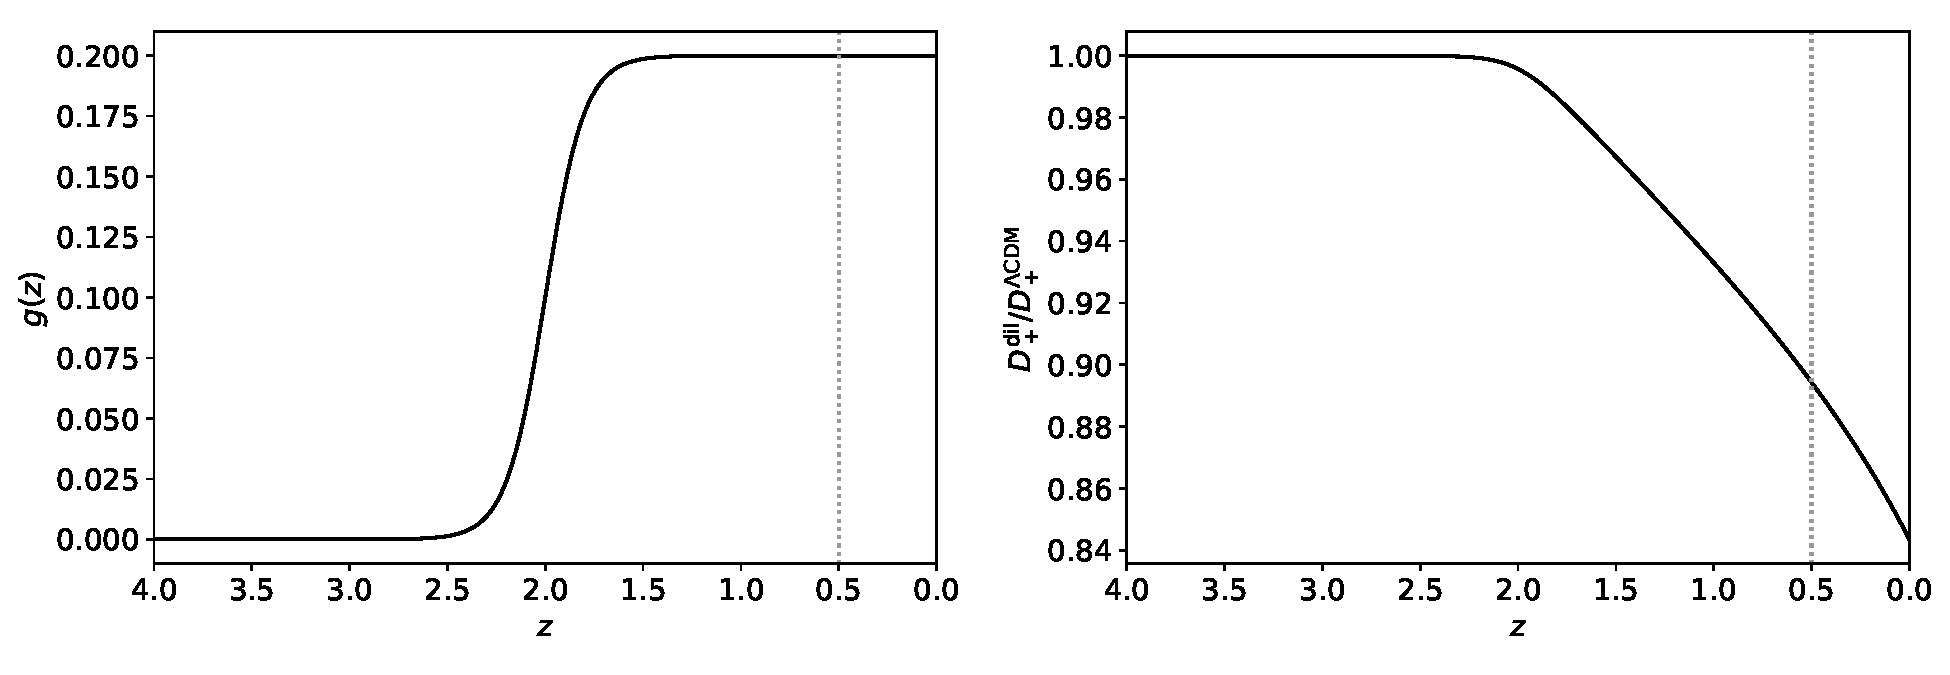
\includegraphics[width=\linewidth]{crecimiento.pdf}
                \caption{El eje horizontal va de $z$ alto a $z$ bajo, de modo que el tiempo avanza hacia la derecha. A la izquierda, la tasa de dilución $g(z)$ del \emph{toy model} con $g_0 = 0.2$, $z_t = 2$ y $\Delta z = 0.2$; se puede ver cómo la tangente hiperbólica prende la dilución alrededor de $z_t$. A la derecha, el cociente entre los factores de crecimiento con y sin dilución, que se separa de $1$ en cuanto $g$ se activa. La línea punteada marca $z = 0.5$, donde se hace todo el análisis.}
                \label{fig:crecimiento}
            \end{figure}

    %=====================================================================%
    \section{Motivación estadística}\label{sec:estadistica}
    %=====================================================================%

        \subsection{Importancia de la covarianza}

            En la práctica, las restricciones cosmológicas que se obtienen de $\xi(r)$ vienen de comparar el vector medido en \emph{bins} de separación, $\hat{\boldsymbol\xi}$, con un modelo $\boldsymbol\xi(\theta)$ mediante una verosimilitud gaussiana:

            \begin{equation}\label{eq:chi2}
                \chi^2(\theta) = \qty[\hat{\boldsymbol\xi} - \boldsymbol\xi(\theta)]^{\rm T}\, \vb{C}^{-1}\, \qty[\hat{\boldsymbol\xi} - \boldsymbol\xi(\theta)],
            \end{equation}

            donde $\vb{C}$ es la matriz de covarianza del estimador. Es esta matriz la que fija el tamaño de las barras de error y qué tan correlacionados están los \emph{bins} entre sí. Lo usual es calcularla una sola vez para una cosmología fiducial, ya sea con simulaciones o con un modelo analítico, y suponer que no depende de los parámetros. Sin embargo, la covarianza sí depende de la cosmología \cite{steele_smith}, y la forma en la que se modela puede afectar las conclusiones que se sacan de los mismos datos de DESI que motivan este trabajo \cite{kolonia}.

            En el caso del modelo de dilución, esto se traduce en tres preguntas concretas. La primera es cuánto cambia la covarianza con la dilución: si $\xi_{\rm dil} \simeq 0.8\,\xi_{\LCDM}$, uno esperaría que la covarianza también baje, y si el cambio resulta pequeño, una covarianza calculada en $\LCDM$ serviría para poner a prueba la dilución; si no, habría que recalcularla para cada $g_0$. La segunda es qué estimador conviene usar, ya que cada uno responde distinto al ruido de los catálogos aleatorios y la respuesta puede depender de la geometría. La tercera es si la diferencia entre modelos es detectable, porque $\xi_{\LCDM} - \xi_{\rm dil} = 0.2\,\xi_{\LCDM}$ solo tiene sentido si se compara con la dispersión del estimador.

            Hay un detalle más que justifica el método. Una sola caja da un solo $\hat\xi(r)$, que es un promedio sobre el volumen de esa caja, mientras que la covarianza es una propiedad del ensamble, y la diferencia entre ambos promedios puede ser importante a escalas grandes \cite{mukherjee}. Por esto, la forma de medir la covarianza es generar muchas realizaciones independientes y ver cómo se dispersan los estimadores entre ellas.

        \subsection{Estimadores de la función de correlación}

            Para medir $\xi(r)$ en un catálogo de $N_D$ puntos (D) se necesita un catálogo aleatorio de referencia (R) con $N_R = \alpha N_D$ puntos uniformes. La idea es contar cuántos pares hay a cada separación y compararlos con los que habría si los puntos no estuvieran correlacionados. Con $\DD(r)$, $\DR(r)$ y $\RR(r)$ se denotan los pares en cada \emph{bin}, normalizados por el número total de pares: $N_D(N_D-1)$, $N_DN_R$ y $N_R(N_R-1)$, respectivamente. Los cuatro estimadores que se comparan son

            \begin{equation}\label{eq:estimadores}
                \hat\xi_{\rm PH} = \frac{\DD}{\RR} - 1, \qquad
                \hat\xi_{\rm DP} = \frac{\DD}{\DR} - 1, \qquad
                \hat\xi_{\rm Ham} = \frac{\DD\,\RR}{\DR^2} - 1, \qquad
                \hat\xi_{\rm LS} = \frac{\DD - 2\DR + \RR}{\RR},
            \end{equation}

            propuestos por Peebles y Hauser \cite{peebles_hauser}, Davis y Peebles \cite{davis_peebles}, Hamilton \cite{hamilton} y Landy y Szalay \cite{landy_szalay}, respectivamente. La diferencia entre ellos está en cómo usan el catálogo aleatorio. Landy y Szalay mostraron que su estimador corrige a primer orden los efectos de borde y tiene una varianza casi poissoniana \cite{landy_szalay}; el de Hamilton tiene propiedades parecidas \cite{hamilton}. Por eso, al compararlos en catálogos con bordes, Landy--Szalay y Hamilton resultan los de mejor desempeño a escalas grandes \cite{kerscher}.

            Es importante notar que en una caja periódica no hay bordes, así que esa ventaja no está garantizada. Además, en una caja periódica $\RR$ se conoce analíticamente, $\RR_i = V_i/V$, con $V_i$ el volumen de la cáscara del \emph{bin} $i$ y $V$ el de la caja. Aun así, en este trabajo se usan catálogos aleatorios, como se haría con un catálogo real, y se usa el mismo catálogo aleatorio en todas las realizaciones. Esta última decisión va a ser importante en los resultados.

            El valor esperado de todos los estimadores es la función de correlación lineal,

            \begin{equation}\label{eq:xi_teo}
                \xi(r) = \int_0^\infty \frac{k^2\,\dd k}{2\pi^2}\, P(k)\, j_0(kr),
            \end{equation}

            con $j_0(x) = \sin x/x$. Para un campo gaussiano, toda su estadística está contenida en $P(k)$ o, de forma equivalente, en $\xi(r)$.

        \subsection{Covarianza muestral}

            Dadas $N$ realizaciones independientes, la covarianza de un estimador se estima como

            \begin{equation}\label{eq:cov_muestral}
                \hat C_{ij} = \frac{1}{N-1}\sum_{s=1}^{N} \qty(\hat\xi_{s,i} - \bar\xi_i)\qty(\hat\xi_{s,j} - \bar\xi_j), \qquad
                r_{ij} = \frac{\hat C_{ij}}{\sqrt{\hat C_{ii}\,\hat C_{jj}}},
            \end{equation}

            donde $\bar\xi_i$ es el promedio sobre las realizaciones y $r_{ij}$ es la matriz de correlación, que normaliza la covarianza para que la diagonal valga $1$ y fuera de ella se lea directamente qué tan correlacionados están dos \emph{bins}. Como $\hat C$ se construye con un número finito de realizaciones, también tiene ruido. Si los $\hat\xi$ siguen una distribución gaussiana, cada elemento tiene una varianza $(C_{ij}^2 + C_{ii}C_{jj})/(N-1)$, por lo que el error relativo de la diagonal es $\sqrt{2/(N-1)}$ y el ruido de $r_{ij}$ fuera de la diagonal es del orden de $1/\sqrt N$.

            El problema empeora al invertirla, que es justo lo que pide la ecuación \eqref{eq:chi2}: $\hat C^{-1}$ está sesgada y hay que corregirla con un factor $(N - n_b - 2)/(N-1)$, donde $n_b$ es el número de \emph{bins} \cite{hartlap}. Con los $n_b = 26$ \emph{bins} de este trabajo, el factor vale $0.73$ para $N = 100$ y $0.9995$ para $N = 5\times10^4$. Dicho de otra forma, con 100 realizaciones la inversa de la covarianza estaría sobrestimada en un 37\% y la precisión que se le asignaría a los parámetros sería demasiado optimista.

        \subsection{Covarianza gaussiana}

            Para tener una idea de qué esperar, conviene ver la forma analítica de la covarianza. Para un campo gaussiano muestreado con ruido de Poisson de densidad $\bar n$ en un volumen $V$, la covarianza de $\hat\xi$ es \cite{grieb, wang_cov}

            \begin{equation}\label{eq:cov_gauss}
                C_{ij} = \frac{1}{\pi^2 V}\int_0^\infty \dd k\, k^2 \qty[P(k) + \frac{1}{\bar n}]^2 \bar\jmath_0(kr_i)\,\bar\jmath_0(kr_j), \qquad
                \bar\jmath_0(kr_i) = \frac{4\pi}{V_i}\int_{\rm bin\ \it i} r^2 j_0(kr)\,\dd r,
            \end{equation}

            donde $\bar\jmath_0$ es $j_0$ promediada en el \emph{bin}. Lo interesante de esta expresión aparece al desarrollar el cuadrado, porque la covarianza se separa en tres términos,

            \begin{equation}\label{eq:cov_terminos}
                C_{ij} = C_{ij}^{PP} + C_{ij}^{PN} + C_{ij}^{NN},
            \end{equation}

            proporcionales a $P^2$, a $2P/\bar n$ y a $1/\bar n^2$, respectivamente. El primero es la varianza cósmica, que viene de tener un volumen finito; el último es el ruido de Poisson, que viene de tener un número finito de puntos, y el de en medio es un término cruzado entre ambos. El ruido de Poisson tiene, además, una forma muy sencilla, porque solo contribuye a la diagonal:

            \begin{equation}\label{eq:cov_poisson}
                C_{ij}^{NN} = \delta_{ij}\,\frac{2}{\bar n^2\, V\, V_i},
            \end{equation}

            que no es otra cosa que el inverso del número esperado de pares en el \emph{bin} $i$. Estas expresiones suponen un número infinito de puntos aleatorios y no incluyen la parte no gaussiana, así que aquí no se usan para comparar elemento a elemento, sino solo para predecir cómo escala la covarianza con la dilución.

        \subsection{Predicciones}\label{sec:predicciones}

            Con todo lo anterior ya se puede predecir lo que se debería ver en el estudio estadístico. Sea $A \equiv P_{\rm dil}/P_{\LCDM} = 0.80$. Al reemplazar $P \to AP$ en la ecuación \eqref{eq:cov_gauss}, cada término escala distinto:

            \begin{equation}\label{eq:cov_dil}
                C_{ij}^{\rm dil} = A^2\, C_{ij}^{PP} + A\, C_{ij}^{PN} + C_{ij}^{NN}.
            \end{equation}

            La primera predicción es la más directa: el promedio de los estimadores con dilución debe ser $A$ veces el de $\LCDM$, $\langle\hat\xi\rangle_{\rm dil} = A\,\xi_{\LCDM}$, con la misma forma y el pico BAO en la misma posición.

            La segunda tiene que ver con cuánto baja la varianza. Si solo hubiera varianza cósmica, el cociente $R_i \equiv C_{ii}^{\rm dil}/C_{ii}^{\LCDM}$ sería $A^2 = 0.64$; si solo hubiera ruido de Poisson, sería $1$. Lo que se espera es algo en medio, y para saber hacia qué lado basta comparar $\bar nP(k)$ con $1$. Con $\bar n = 5\times10^{-5}\,h^3\,\mathrm{Mpc}^{-3}$ se tiene $1/\bar n = 2\times10^4\,(\hMpc)^3$, mientras que el máximo de $P_L$ en $z = 0.5$ es $1.4\times10^4\,(\hMpc)^3$, en $k = 0.017\,h\,\mathrm{Mpc}^{-1}$. Es decir, $\bar nP \leq 0.69$ en todas las escalas y $\bar nP \leq 0.16$ para $k \geq 0.1\,h\,\mathrm{Mpc}^{-1}$, así que el ruido domina y $R_i$ debe quedar mucho más cerca de $1$ que de $0.64$. Además, el ruido de los catálogos aleatorios tampoco se diluye, por lo que los estimadores que más lo cargan deben dar un $R_i$ todavía más cercano a $1$.

            La tercera es sobre la correlación entre \emph{bins}. Como $C^{NN}$ solo vive en la diagonal, fuera de ella únicamente quedan los términos que sí se diluyen, $C_{ij}^{\rm dil} = A^2C_{ij}^{PP} + A\,C_{ij}^{PN}$ para $i \neq j$. La diagonal casi no cambia, así que la dilución debe debilitar la correlación entre \emph{bins}, reduciendo $r_{ij}$ por un factor entre $A^2/R$ y $A/R$.

            La cuarta compara a los estimadores entre sí. Como el catálogo aleatorio es el mismo en todas las realizaciones, $\RR$ no cambia y no aporta varianza. En el límite de Poisson y con $\xi \ll 1$, las fluctuaciones relativas de $\DD$ y $\DR$ son independientes, con varianzas $2\sigma_0^2$ y $\sigma_0^2/\alpha$, donde $\sigma_0^2 = V/(N_D^2V_i)$. El factor $2$ aparece porque con $N_D$ puntos solo hay $N_D^2/2$ pares distintos, mientras que entre D y R hay $N_DN_R$. Al linealizar las ecuaciones \eqref{eq:estimadores}, las fluctuaciones de cada estimador son $\delta\hat\xi_{\rm PH} \simeq \delta\DD$, $\delta\hat\xi_{\rm DP} \simeq \delta\DD - \delta\DR$ y $\delta\hat\xi_{\rm Ham} \simeq \delta\hat\xi_{\rm LS} \simeq \delta\DD - 2\,\delta\DR$, por lo que

            \begin{equation}\label{eq:var_poisson}
                {\rm Var}[\hat\xi_{\rm PH}] : {\rm Var}[\hat\xi_{\rm DP}] : {\rm Var}[\hat\xi_{\rm LS}] = 2 : \qty(2 + \frac{1}{\alpha}) : \qty(2 + \frac{4}{\alpha}).
            \end{equation}

            Es decir, respecto a Landy--Szalay, Peebles--Hauser debe tener $\alpha/(\alpha+2)$ de su varianza y Davis--Peebles $(2\alpha+1)/(2\alpha+4)$: $0.33$ y $0.50$ para $\alpha = 1$, y $0.60$ y $0.70$ para $\alpha = 3$. La varianza cósmica entra solo en $\DD$ y le suma lo mismo a los cuatro estimadores, digamos $c\,\sigma_0^2$, así que los cocientes medidos deberían quedar un poco por encima de estos valores; por ejemplo, ${\rm Var}[\hat\xi_{\rm PH}]/{\rm Var}[\hat\xi_{\rm LS}] = (2 + c)/(2 + 4/\alpha + c)$. Cuando $\alpha \to \infty$ los cuatro coinciden. Además, como $c$ es justo la parte que se diluye, con dilución debe bajar a un valor entre $A^2c$ y $Ac$, según pese más $C^{PP}$ o $C^{PN}$, y con él los cocientes deben bajar un poco hacia la estimación de Poisson.

            La quinta predicción es un efecto secundario de usar siempre el mismo catálogo aleatorio. El error de muestreo de $\RR$, $\epsilon_i = \RR_i/(V_i/V) - 1$, es el mismo en todas las realizaciones, así que no se promedia y se queda como un sesgo: $\langle\hat\xi_{\rm PH}\rangle \simeq \xi - \epsilon$, mientras que $\langle\hat\xi_{\rm Ham}\rangle \simeq \langle\hat\xi_{\rm LS}\rangle \simeq \xi + \epsilon$, con el signo contrario. Davis--Peebles se salva porque no usa $\RR$, y $\DR$, aunque también usa el catálogo fijo, sí se promedia: en una caja periódica, al mover los puntos de D de una realización a otra, su valor esperado es exactamente $V_i/V$. El tamaño típico del sesgo es $\epsilon \sim \sqrt{2V/(N_R^2V_i)}$ y, a diferencia del ruido, no baja al aumentar $N$.

    %=====================================================================%
    \section{Metodología}\label{sec:metodologia}
    %=====================================================================%

        Todo el análisis está escrito en Python con NumPy \cite{numpy} y SciPy \cite{scipy}. CLASS \cite{class} se usa únicamente para obtener el fondo y el espectro lineal de $\LCDM$; el resto del código, es decir, el crecimiento con dilución, los campos, los catálogos, los estimadores y las covarianzas, es propio. Gran parte de lo que se hace aquí es una extensión de lo visto en las prácticas del curso: la generación de campos gaussianos sigue la práctica 3 y los estimadores de $\xi(r)$, la práctica 5. Los parámetros usados se resumen en la Tabla~\ref{tab:parametros}.

        \begin{table}[H]
            \centering
            \caption{Parámetros de las simulaciones.}
            \label{tab:parametros}
            \begin{tabular}{ll}
                \toprule
                Parámetro & Valor \\
                \midrule
                Cosmología ($\LCDM$ plano) & $\Omega_{m0} = 0.3$, $\Omega_{b0} = 0.045$, $h = 0.7$, $n_s = 0.965$, $\sigma_8 = 0.8$ \\
                \emph{Toy model} & $g_0 \in \{0, 0.2\}$, $z_t = 2$, $\Delta z = 0.2$ \\
                \emph{Redshift} & $z = 0.5$ \\
                Caja & $L = 1000\,\hMpc$, malla $128^3$ (celdas de $7.8\,\hMpc$) \\
                Densidad de puntos & $\bar n = 5\times10^{-5}\,h^3\,\mathrm{Mpc}^{-3}$ ($N_D \simeq 5\times10^4$) \\
                Catálogos aleatorios & $\alpha = N_R/N_D \in \{1, 3\}$ \\
                \emph{Bins} de separación & $20$--$150\,\hMpc$, $\Delta r = 5\,\hMpc$ ($26$ \emph{bins}) \\
                Realizaciones & $N = 5\times10^4$ por modelo \\
                \bottomrule
            \end{tabular}
        \end{table}

        \subsection{Crecimiento y espectro con dilución}

            El primer paso es obtener $P_{\rm dil}$. CLASS da el fondo, $H(z)$ y $\Omega_m(z)$, que es el mismo para los dos modelos, y el espectro lineal $P_L(k)$ en $z = 0.5$. La ecuación \eqref{eq:crecimiento_lna} se integra en $\ln a$ con \texttt{solve\_ivp}, con tolerancias \texttt{rtol = 1e-10} y \texttt{atol = 1e-13}, desde $z = 99$ hasta $z = 0$. Se escogió $z = 99$ porque ahí $g$ todavía es cero, de modo que las condiciones iniciales se pueden tomar directamente de CLASS: $D_+$ y $f$ en ese \emph{redshift}.

            Antes de usar el resultado conviene comprobar que funciona. Con $g_0 = 0$ se recupera el $D_+$ de CLASS con una diferencia relativa máxima de $2\times10^{-9}$ en $z \in \{0, 0.5, 1, 2, 5\}$. Con $g_0 = 0.2$ se obtiene $P_{\rm dil}/P_{\LCDM} = 0.7999$ en $z = 0.5$, y con esto se construye $P_{\rm dil}$ mediante la ecuación \eqref{eq:pdil}.

        \subsection{Campos gaussianos y catálogos}

            El campo se genera en una caja periódica de lado $L = 1000\,\hMpc$ con una malla de $128^3$ celdas, cada una de volumen $V_{\rm celda}$. A diferencia de las prácticas, donde había que imponer a mano la condición de realidad sobre las amplitudes y fases en Fourier, aquí se parte de ruido blanco real $w$ en la malla y se colorea en el espacio de Fourier:

            \begin{equation}\label{eq:campo}
                \delta(\vb{k}) = \sqrt{\frac{P(k)}{V_{\rm celda}}}\ \mathrm{FFT}[w](\vb{k}).
            \end{equation}

            La ventaja de hacerlo así es que, como $w$ es real, la condición $\delta(-\vb{k}) = \delta^*(\vb{k})$ se cumple sola. El modo $\vb{k} = 0$ se fija en cero. Para comprobar que el campo tiene el espectro correcto, se promedia $|\delta(\vb{k})|^2$ en cáscaras de $\Delta k = 0.01\,h\,\mathrm{Mpc}^{-1}$ sobre 20 realizaciones: el resultado sigue a $P_{\rm dil}$ a menos del 1\%, salvo en el primer \emph{bin}, que tiene muy pocos modos (Figura~\ref{fig:validacion}).

            \begin{figure}[H]
                \centering
                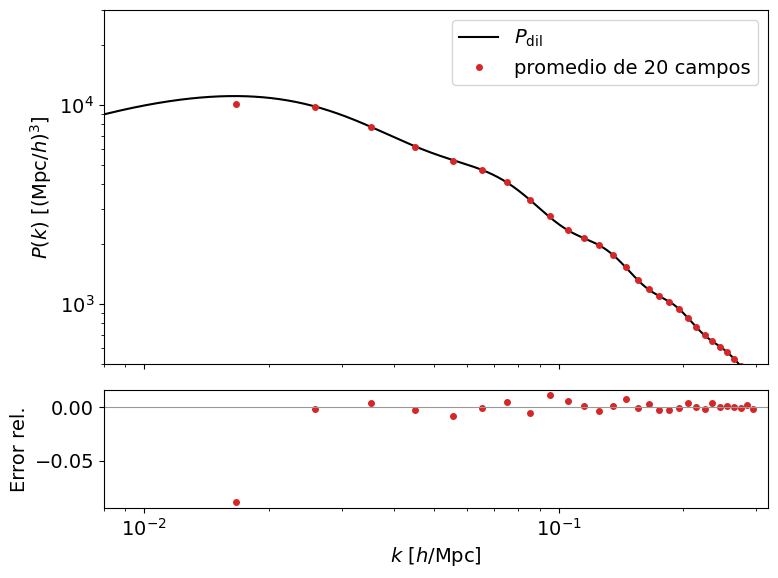
\includegraphics[width=0.6\linewidth]{validacion_pk.png}
                \caption{Promedio de $|\delta(\vb{k})|^2$ sobre 20 campos con $g_0 = 0.2$ (puntos rojos) comparado con $P_{\rm dil}(k)$ (línea negra). El panel de abajo muestra el error relativo, que se mantiene por debajo del 1\% salvo en el primer \emph{bin}, donde hay muy pocos modos.}
                \label{fig:validacion}
            \end{figure}

            El siguiente problema es pasar del campo a puntos. Un $\delta$ gaussiano puede tomar valores menores que $-1$, lo que daría densidades negativas, así que para la densidad se usa la transformación lognormal $1 + \delta \to e^{\delta - \sigma^2/2}$ \cite{coles_jones}, donde $\sigma^2$ es la varianza del campo en la malla y el término $-\sigma^2/2$ asegura que la densidad media no cambie. Después, en cada celda se pone un número de puntos con distribución de Poisson de media $\bar n\, V_{\rm celda}\, e^{\delta - \sigma^2/2}$, en posiciones uniformes dentro de la celda. Con $\bar n = 5\times10^{-5}\,h^3\,\mathrm{Mpc}^{-3}$, cada catálogo tiene unos $5\times10^4$ puntos; en la realización de prueba se obtuvieron $N_D = 50\,049$, contra los $\bar n V = 50\,000$ esperados. La Figura~\ref{fig:campo} muestra un corte del campo y del catálogo correspondiente.

            \begin{figure}[H]
                \centering
                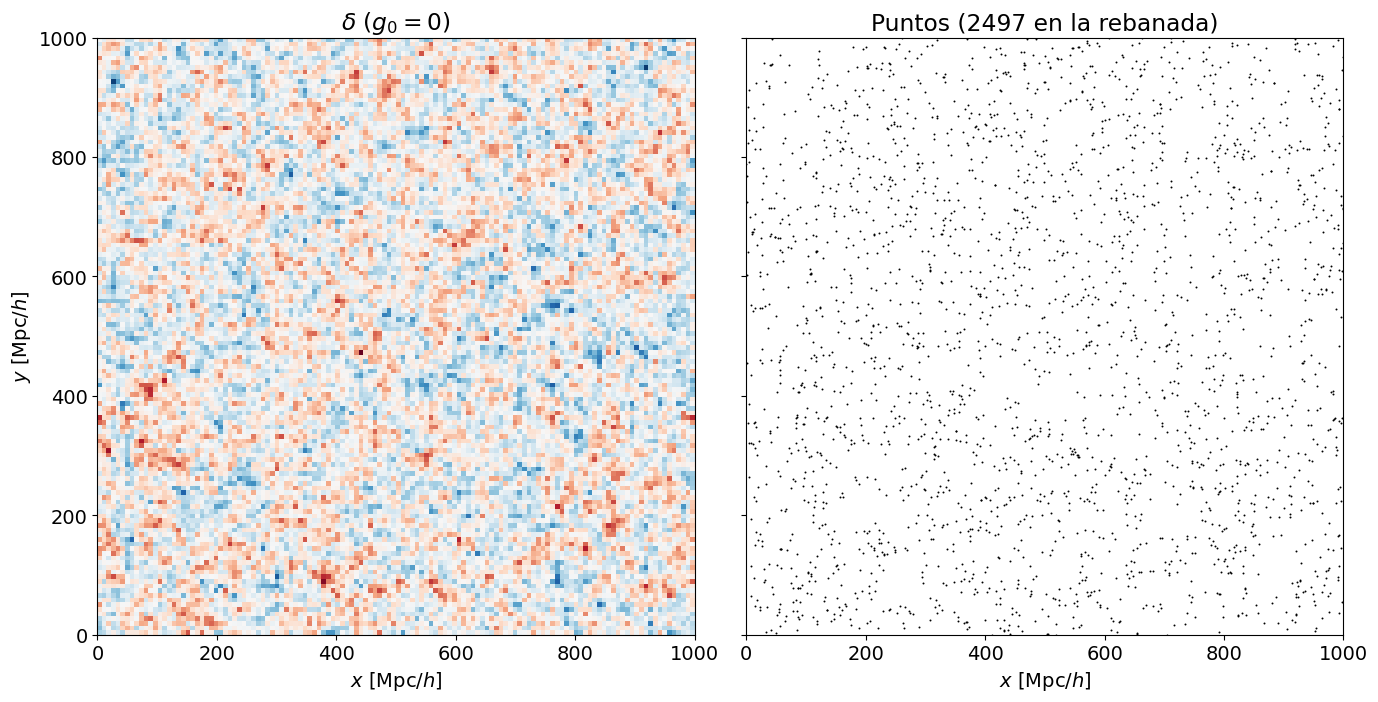
\includegraphics[width=\linewidth]{campo_puntos.png}
                \caption{A la izquierda, un corte de ${\sim}50\,\hMpc$ de grosor del campo $\delta$ con $g_0 = 0$, donde el rojo representa sobredensidades y el azul subdensidades. A la derecha, los puntos del catálogo que caen en el mismo corte.}
                \label{fig:campo}
            \end{figure}

            Por último, los catálogos aleatorios tienen $N_R = \alpha N_D$ puntos uniformes, con $\alpha = 1$ y $3$. Se genera uno para cada $\alpha$ y se usa el mismo en todas las realizaciones, así que $\RR$ se calcula una sola vez y se ahorra una buena parte del tiempo de cómputo.

        \subsection{Conteo de pares y estimadores}

            Contar pares es, por mucho, la parte más cara del cálculo. Para hacerlo de forma eficiente se usa \texttt{scipy.spatial.cKDTree}, que organiza los puntos en un árbol y permite contar vecinos sin comparar todos los pares entre sí; la opción \texttt{boxsize=L} se encarga de las condiciones periódicas. El método \texttt{count\_neighbors} devuelve el número acumulado de pares hasta cada borde, así que los conteos por \emph{bin} salen de restar bordes consecutivos. Los \emph{bins} van de $20$ a $150\,\hMpc$ con $\Delta r = 5\,\hMpc$, un rango escogido para que incluya el pico BAO en ${\sim}105\,\hMpc$. Con $\DD$, $\DR$ y $\RR$ se evalúan los cuatro estimadores de la ecuación \eqref{eq:estimadores}.

            Para comparar, el $\xi(r)$ teórico se calcula con la ecuación \eqref{eq:xi_teo} mediante la regla del trapecio. Se le agrega un factor $e^{-k^2}$, con $k$ en $h\,\mathrm{Mpc}^{-1}$, que solo sirve para que la integral converja y no cambia el resultado para $r \geq 20\,\hMpc$.

        \subsection{Realizaciones y cómputo en paralelo}\label{sec:realizaciones}

            Cada realización usa una semilla $s$ para todos sus números aleatorios: el ruido blanco, los conteos de Poisson y las posiciones dentro de las celdas. La misma semilla se usa para $g_0 = 0$ y $g_0 = 0.2$, así que los dos modelos parten del mismo ruido blanco y sus campos gaussianos son proporcionales, $\delta_{\rm dil} = \sqrt{A}\,\delta_{\LCDM}$. Lo que no comparten es el ruido de Poisson: la cantidad de números aleatorios que gasta cada sorteo depende de la media de la celda, así que el generador se desfasa en cuanto los conteos de los dos modelos difieren y, a partir de ahí, los conteos y las posiciones son prácticamente independientes. De hecho, la correlación entre los $\hat\xi$ de los dos modelos con la misma semilla es de apenas $0.04$--$0.08$ por \emph{bin}, así que, para la comparación entre modelos, la semilla común casi no reduce el ruido. Para que el ruido de Poisson también fuera común habría que sacar los dos catálogos de uno solo, quedándose con cada punto con una probabilidad que depende del modelo (catálogos anidados).

            El plan original era usar entre 60 y 100 realizaciones por modelo, pero con 100 realizaciones el error de cada varianza es de ${\sim}14\%$, demasiado grande para ver diferencias de unos cuantos por ciento. El problema es que una realización tarda unos $10.5\,\mathrm{s}$, casi todo en el conteo de pares. Para resolverlo, las realizaciones se reparten entre procesos con \texttt{multiprocessing.Pool} y las corridas grandes se hicieron en un nodo de CPU de NERSC con 256 procesos, desde un trabajo de Slurm que ejecutaba sin interfaz (\texttt{jupyter nbconvert}) una copia del \emph{notebook}, con el número de realizaciones y de procesos como variables de entorno. Ese código de producción se reemplazó después por \texttt{slurm/farm.py}, que tiene las mismas funciones y, con la opción \texttt{-{}-independientes}, reproduce bit a bit los resultados de este trabajo. La corrida final, con $N = 5\times10^4$ realizaciones por modelo ($10^5$ en total), tardó $14\,403\,\mathrm{s}$, unas 4 horas, cuando en serie habría tardado unos 12 días.

            También se hicieron corridas con $N = 10^3$, $5\times10^3$ y $2\times10^4$. Como la realización $s$ siempre usa la semilla $s$, cada corrida coincide exactamente con las primeras $N$ realizaciones de la corrida más grande, cosa que se comprobó; por eso solo se conserva la de $N = 5\times10^4$. Esto resultó muy útil, porque permite estudiar la convergencia con $N$ usando subconjuntos de la corrida final, con errores estimados por \emph{bootstrap} sobre las realizaciones (200 remuestreos).

        \subsection{Estructura del código}

            El código está pensado como una cadena de funciones, una por cada paso del flujo de la Figura~\ref{fig:flujo}, siguiendo la idea de que cada una consume lo que produce la anterior. La primera, \texttt{crecimiento(g0)}, integra la ecuación \eqref{eq:crecimiento_lna} con ayuda de \texttt{g} y \texttt{dg}, el \emph{toy model} y su derivada, y devuelve $D_+(z)$. Con el espectro ya construido, \texttt{campo\_gaussiano(Pk, rng)} genera $\delta$ en la malla y \texttt{puntos(delta, rng)} aplica la transformación lognormal y el muestreo de Poisson para devolver el catálogo. Después, \texttt{pares(A)} cuenta los pares dentro de un mismo catálogo, $\DD$ o $\RR$, y \texttt{pares(A, B)} los pares entre dos catálogos, $\DR$, ya normalizados; el diccionario \texttt{EST} contiene los cuatro estimadores. Todo esto se une en \texttt{realizacion(s, g0)}, que, dada una semilla y un modelo, devuelve $\hat\xi$ para cada estimador y cada $\alpha$. Por último, \texttt{xi\_teo(Pk)} evalúa la ecuación \eqref{eq:xi_teo} para comparar.

            Con esta estructura, cambiar un paso no obliga a tocar los demás. Los resultados se guardan en archivos \texttt{.npz}, con una matriz de $N \times 26$ por cada combinación de modelo, estimador y $\alpha$, y todo lo demás se calcula después a partir de esos archivos, sin repetir las realizaciones: \texttt{covarianza.ipynb} produce las figuras y los números de la Sección~\ref{sec:resultados}, incluido el estudio de convergencia. La Figura~\ref{fig:directorio} muestra cómo están organizados los archivos del proyecto.

            \begin{figure}[H]
                \centering
                \resizebox{\linewidth}{!}{%
                \begin{tikzpicture}[
                    box/.style = {draw, thick, rounded corners=2pt, fill=black!4, align=center,
                                  minimum height=1.3cm, text width=2.3cm, font=\small},
                    ext/.style = {box, dashed, fill=white},
                    fn/.style  = {font=\scriptsize\ttfamily, text=black!70},
                    arr/.style = {-{Stealth}, thick}
                  ]
                    \node[box] (toy)   at (0,0)  {\emph{Toy model}\\$g(z)$};
                    \node[box] (ode)   at (3,0)  {Crecimiento\\$D_+(z)$};
                    \node[box] (pdil)  at (6,0)  {Espectro\\$P_{\rm dil}(k)$};
                    \node[box] (field) at (9,0)  {Campo y\\catálogo};
                    \node[box] (est)   at (12,0) {Estimadores\\$\hat\xi(r)$};
                    \node[box] (cov)   at (15,0) {Covarianza\\$\hat C_{ij}$};
                    \node[ext] (class) at (4.5,-2.6) {CLASS};

                    \node[fn, below=2pt of toy]   {g, dg};
                    \node[fn, below=2pt of ode] (fode) {crecimiento};
                    \node[fn, below=2pt of field, align=center] {campo\_gaussiano\\puntos};
                    \node[fn, below=2pt of est, align=center]   {pares\\EST};
                    \node[fn, below=2pt of cov]   {np.cov};

                    \draw[arr] (toy) -- (ode);
                    \draw[arr] (ode) -- (pdil);
                    \draw[arr] (pdil) -- (field);
                    \draw[arr] (field) -- (est);
                    \draw[arr] (est) -- (cov);
                    \draw[arr] (class.north west) -- node[left, font=\small] {$H(z)$, $\Omega_m(z)$} (fode.south);
                    \draw[arr] (class.north east) -- node[right, font=\small] {$P_L(k)$} (pdil.south);
                    \draw[arr] (est.north) to[out=135, in=45, looseness=1.1]
                        node[above, font=\small] {$N$ realizaciones: \texttt{realizacion(s, g0)}} (field.north);
                \end{tikzpicture}}
                \caption{Flujo del código. Cada caja es un paso y debajo de ella está la función que lo implementa. CLASS entra solo al principio, con el fondo y el espectro lineal; el ciclo entre el campo y los estimadores se repite para cada semilla $s$ y cada $g_0$.}
                \label{fig:flujo}
            \end{figure}

            \begin{figure}[H]
                \centering
                \begin{minipage}{0.92\linewidth}
                \dirtree{%
                    .1 proyecto/.
                    .2 plan\_proyecto.md\DTcomment{plan y parámetros del proyecto}.
                    .2 covarianza\_test.ipynb\DTcomment{desarrollo y pruebas con $N = 100$}.
                    .2 covarianza.ipynb\DTcomment{análisis de la corrida final: figuras, números y convergencia}.
                    .2 data/.
                    .3 xi\_estimadores.npz\DTcomment{$\hat\xi$ de la corrida de prueba}.
                    .2 slurm/.
                    .3 farm.py\DTcomment{código de producción (el que corre en Slurm)}.
                    .3 farm.sbatch\DTcomment{trabajo de Slurm}.
                    .3 LEEME.md\DTcomment{configuraciones y formato de los datos}.
                    .3 datos/.
                    .4 xi\_estimadores\_N50000.npz\DTcomment{$\hat\xi$ por realización (este trabajo)}.
                    .4 <configuración>/\DTcomment{conteos de pares para extensiones}.
                    .2 references/\DTcomment{artículos de referencia}.
                    .2 presentacion/\DTcomment{presentación}.
                    .2 reporte/\DTcomment{este reporte}.
                }
                \end{minipage}
                \caption{Organización de los archivos del proyecto. El \emph{notebook} de prueba sirvió para construir cada paso con pocas realizaciones; la producción vive en \texttt{slurm/}, donde \texttt{farm.py} usa las mismas funciones y guarda los resultados en archivos \texttt{.npz} que después lee \texttt{covarianza.ipynb}.}
                \label{fig:directorio}
            \end{figure}

    %=====================================================================%
    \section{Resultados}\label{sec:resultados}
    %=====================================================================%

        En los resultados hay, básicamente, tres cosas a las que se les ha prestado atención: si los estimadores reproducen el $\xi(r)$ teórico, cómo se comparan sus covarianzas entre sí y cómo cambia la covarianza con la dilución. Todos los resultados de esta sección corresponden a la corrida con $N = 5\times10^4$ realizaciones por modelo, y la Tabla~\ref{tab:resultados} resume la comparación con las predicciones de la Sección~\ref{sec:predicciones}.

        \subsection{Promedio de los estimadores}

            Lo primero es comprobar que los estimadores miden lo que deben (Figura~\ref{fig:xi_promedio}). Los promedios siguen al $\xi(r)$ teórico, incluido el pico BAO en ${\sim}105\,\hMpc$, y con $g_0 = 0.2$ la amplitud baja sin que cambie la forma, tal como se predijo.

            Con $N = 5\times10^4$, las barras de error del promedio, $\sigma/\sqrt N$, ya son más pequeñas que los puntos, y lo que queda a la vista no es ruido, sino un sesgo. Peebles--Hauser y Landy--Szalay se desvían del teórico con signos contrarios, hasta ${\sim}10\,(\hMpc)^2$ en $r^2\xi$ entre $120$ y $130\,\hMpc$, y lo hacen exactamente igual en los dos modelos. Hamilton coincide con Landy--Szalay, y Davis--Peebles, que no usa $\RR$, sigue al teórico. Esto es justo lo que se esperaba de la quinta predicción: el sesgo viene del error de muestreo del catálogo aleatorio, que es el mismo en todas las realizaciones. Para $\alpha = 3$ y $r \simeq 125\,\hMpc$, la estimación $\epsilon \sim \sqrt{2V/(N_R^2V_i)}$ da $r^2\epsilon \approx 5\,(\hMpc)^2$, del mismo orden que las desviaciones observadas.

            Este sesgo ya se alcanzaba a ver en la corrida de prueba con $N = 100$, porque se repetía igual en los dos modelos, pero es con $N = 5\times10^4$ que queda claro que no es ruido. Aumentar $N$ no lo corrige; para quitarlo hace falta usar más puntos aleatorios, un catálogo aleatorio distinto en cada realización o, en una caja periódica, el $\RR$ analítico.

            \begin{figure}[H]
                \centering
                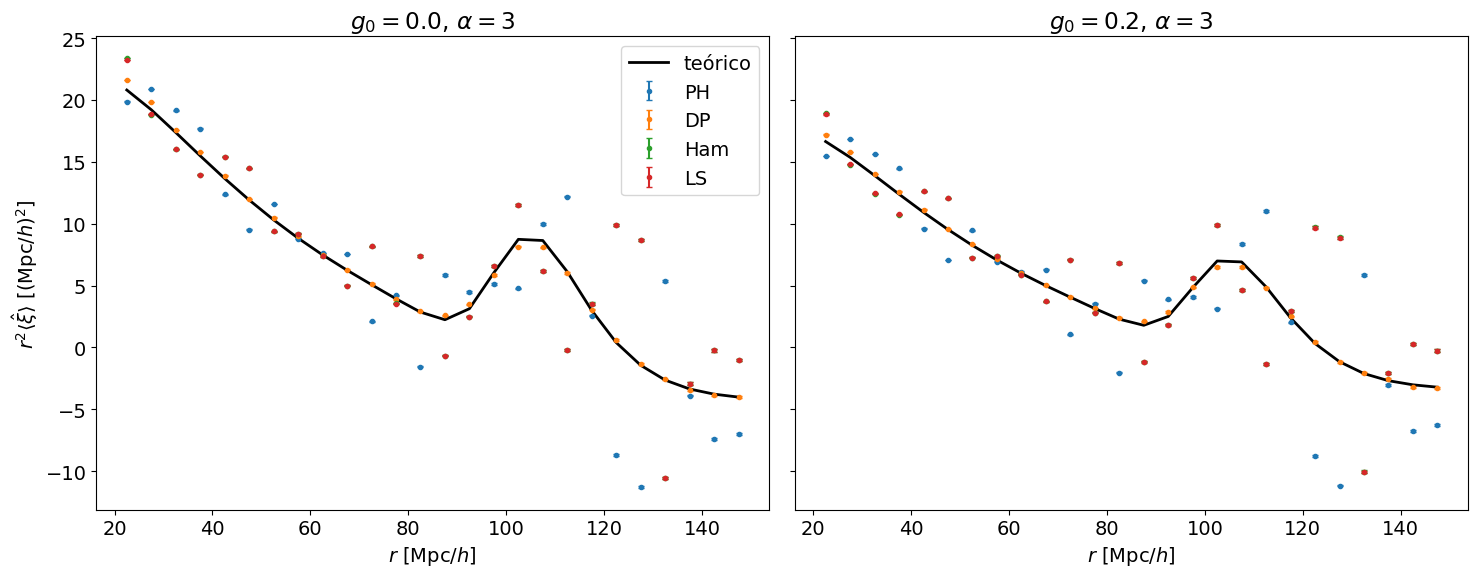
\includegraphics[width=\linewidth]{xi_promedio.png}
                \caption{Promedio de $r^2\hat\xi(r)$ sobre las $5\times10^4$ realizaciones para cada estimador, con $\alpha = 3$, sin dilución (izquierda) y con $g_0 = 0.2$ (derecha). La línea negra es el $\xi(r)$ teórico de la ecuación \eqref{eq:xi_teo}. Las barras de error, $\sigma/\sqrt N$, son más pequeñas que los puntos, así que las desviaciones que se ven, sobre todo entre $120$ y $130\,\hMpc$, no son ruido, sino el sesgo del catálogo aleatorio fijo. Los puntos de Hamilton quedan tapados por los de Landy--Szalay, porque coinciden.}
                \label{fig:xi_promedio}
            \end{figure}

        \subsection{Matrices de correlación}

            Las matrices de correlación (Figura~\ref{fig:correlacion}) son casi diagonales, con una banda positiva junto a la diagonal, es decir, solo los \emph{bins} vecinos están correlacionados de forma apreciable. Para Landy--Szalay, la correlación entre \emph{bins} vecinos es $r_{i,i+1} = 0.129 \pm 0.001$ en $\LCDM$ y $0.104 \pm 0.001$ con dilución. El ruido fuera de la diagonal es de ${\sim}1/\sqrt N \approx 0.004$, así que la diferencia es real y va en la dirección de la tercera predicción: la dilución debilita la correlación entre \emph{bins}.

            El cociente entre ambas, $0.81 \pm 0.01$, cae dentro del intervalo $[A^2/R, A/R] = [0.66, 0.83]$, con $R = 0.965$. Que quede cerca del extremo superior sugiere que, fuera de la diagonal, domina el término cruzado $C^{PN}$, lo que tiene sentido con $\bar nP < 1$.

            \begin{figure}[H]
                \centering
                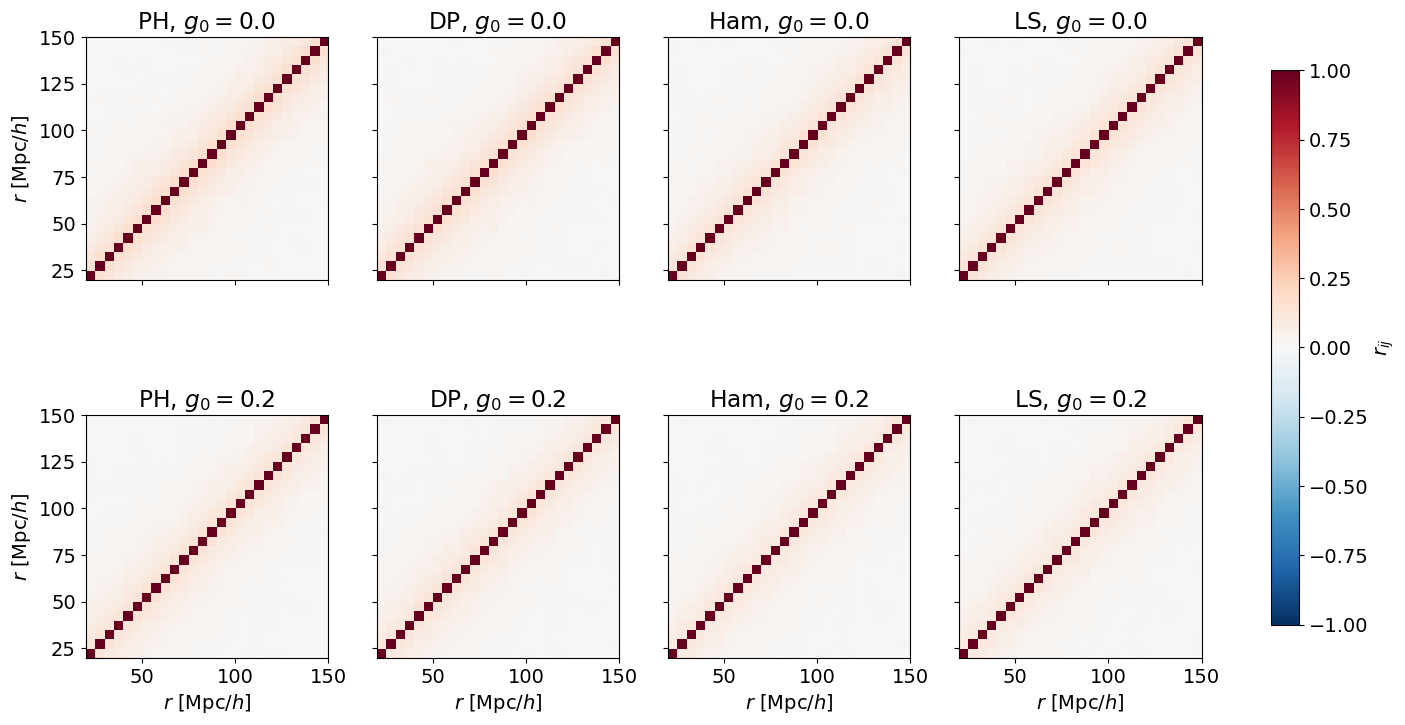
\includegraphics[width=\linewidth]{matrices_correlacion.png}
                \caption{Matrices de correlación $r_{ij}$ de los cuatro estimadores con $\alpha = 3$, sin dilución (arriba) y con $g_0 = 0.2$ (abajo). La diagonal vale $1$ por construcción; la banda rosada a su lado es la correlación entre \emph{bins} vecinos, que se debilita con la dilución.}
                \label{fig:correlacion}
            \end{figure}

        \subsection{Comparación entre estimadores}

            Al comparar los estimadores entre sí (Figura~\ref{fig:var_estimadores}), lo primero que se nota es que los cocientes casi no dependen de $r$. Sin dilución y con $\alpha = 1$, Peebles--Hauser tiene $0.360 \pm 0.001$ de la varianza de Landy--Szalay y Davis--Peebles $0.522$, con un error menor que $0.001$; con $\alpha = 3$, los valores son $0.627 \pm 0.001$ y $0.721$. Con dilución bajan un poco: $0.353$ y $0.517$ con $\alpha = 1$, y $0.620$ y $0.716$ con $\alpha = 3$. Hamilton y Landy--Szalay tienen prácticamente la misma varianza.

            Sin dilución, los cuatro valores quedan entre $0.02$ y $0.03$ por encima de la estimación de Poisson de la cuarta predicción ($0.33$, $0.50$, $0.60$ y $0.70$), justo como se esperaba por la varianza cósmica que comparten. Al despejar $c$ del cociente de Peebles--Hauser se obtiene $c = 0.250$ con $\alpha = 1$ y $c = 0.246$ con $\alpha = 3$, es decir, prácticamente el mismo exceso en los dos casos, como debe ser, porque $\DD$ no depende de $\alpha$. Con dilución, $c$ baja a $0.19$ y $0.17$, dentro del intervalo $[A^2c, Ac] = [0.16, 0.20]$, y eso es lo que hace bajar los cocientes: la predicción es $0.352 \pm 0.002$ para $\alpha = 1$ y $0.620 \pm 0.002$ para $\alpha = 3$, contra $0.353$ y $0.620$ medidos. La razón del orden entre estimadores es sencilla: con el catálogo aleatorio fijo, la varianza de Peebles--Hauser solo viene de $\DD$, Davis--Peebles carga además con el ruido de $\DR$, y Hamilton y Landy--Szalay con cuatro veces ese ruido. Al subir $\alpha$, el ruido de $\DR$ baja y los cocientes se acercan a $1$.

            Este resultado parece contradecir lo que normalmente se dice de Landy--Szalay, pero solo en apariencia. Su ventaja viene de corregir los efectos de borde y, en una caja periódica, no hay bordes que corregir; lo único que queda es el ruido extra de $\DR$, y por eso termina siendo, junto con Hamilton, el estimador con mayor varianza.

            Hay un último detalle en la figura: Hamilton queda unos pocos por ciento por encima de Landy--Szalay en $r \lesssim 50\,\hMpc$. Esto también es del orden esperado, porque en Hamilton el ruido de $\DR$ aparece multiplicado por $(1 + \xi)$, lo que da ${\rm Var}_{\rm Ham}/{\rm Var}_{\rm LS} - 1 \simeq 4\xi/(\alpha+2)$, es decir, ${\sim}0.05$ en el primer \emph{bin} con $\alpha = 1$, donde $\xi \approx 0.04$, y menos a mayor $r$.

            \begin{figure}[H]
                \centering
                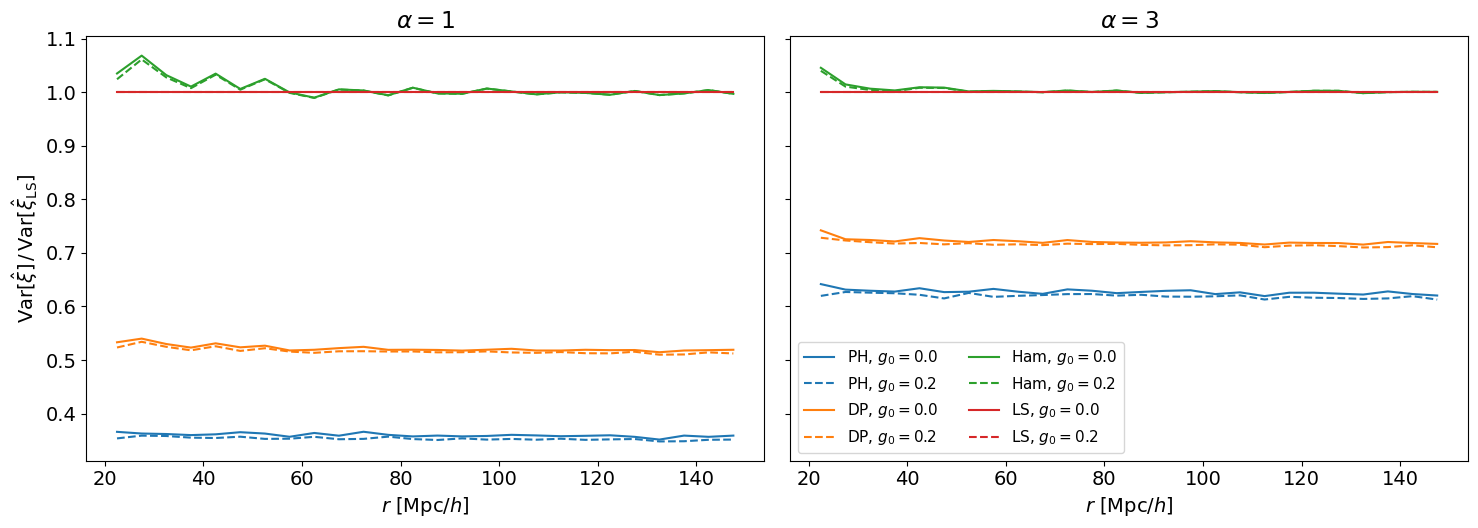
\includegraphics[width=\linewidth]{varianza_estimadores.png}
                \caption{Varianza de cada estimador dividida entre la de Landy--Szalay, para $\alpha = 1$ (izquierda) y $\alpha = 3$ (derecha). Las líneas continuas son para $g_0 = 0$ y las discontinuas para $g_0 = 0.2$. Con dilución, los cocientes de Peebles--Hauser y Davis--Peebles bajan ligeramente (${\sim}0.007$), porque se diluye la varianza cósmica que comparten los cuatro estimadores.}
                \label{fig:var_estimadores}
            \end{figure}

        \subsection{Comparación entre modelos}

            Esta es la comparación que motivó el trabajo (Figura~\ref{fig:cociente}). El cociente de las varianzas con y sin dilución es, en promedio sobre $r$ y con $\alpha = 3$, $0.953 \pm 0.002$ para Peebles--Hauser, $0.958 \pm 0.002$ para Davis--Peebles y $0.965 \pm 0.002$ para Hamilton y Landy--Szalay; con $\alpha = 1$, Hamilton y Landy--Szalay dan $0.970$ y $0.971$. Está entre $0.64$ y $1$, pero mucho más cerca de $1$. Es decir, la segunda predicción se cumple, pero el efecto es mucho más pequeño de lo que uno pensaría al ver que la señal baja un 20\%: con esta densidad de puntos domina el ruido de Poisson, que no se diluye. El orden entre estimadores también coincide con lo predicho, ya que los que cargan más ruido de $\DR$, que tampoco se diluye, son los que quedan más cerca de $1$.

            Por rangos de $r$, Landy--Szalay da $0.970 \pm 0.003$ entre $20$ y $60\,\hMpc$, $0.967 \pm 0.003$ entre $60$ y $100\,\hMpc$ y $0.961 \pm 0.003$ entre $100$ y $150\,\hMpc$, así que, si el cociente depende de $r$, lo hace a lo más en ${\sim}1\%$. En la práctica, esto significa que, con esta densidad de puntos, usar una covarianza de $\LCDM$ para analizar un universo con dilución sobrestimaría las varianzas apenas en un ${\sim}4\%$.

            \begin{figure}[H]
                \centering
                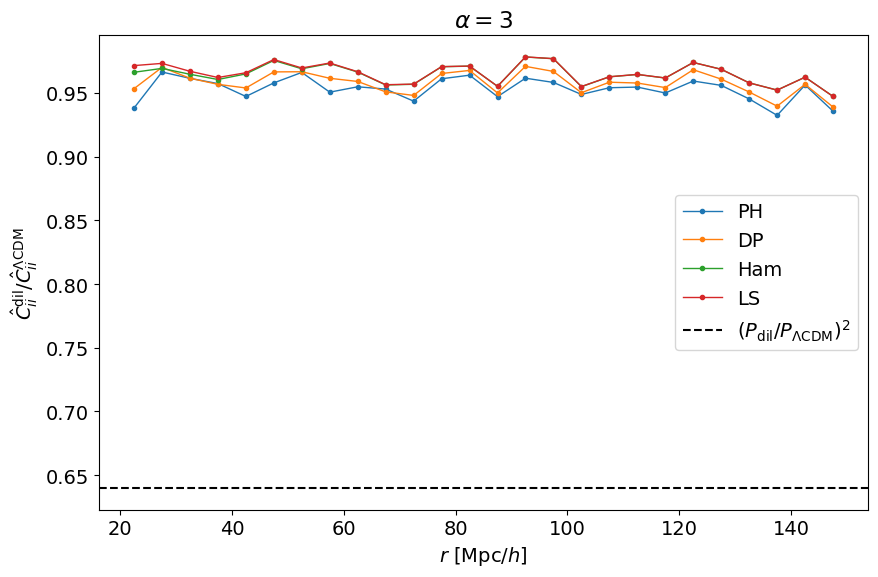
\includegraphics[width=0.65\linewidth]{cociente_modelos.png}
                \caption{Cociente de la diagonal de la covarianza con y sin dilución para los cuatro estimadores, con $\alpha = 3$. La línea discontinua es $(P_{\rm dil}/P_{\LCDM})^2 = 0.64$, es decir, el valor que se tendría si solo hubiera varianza cósmica.}
                \label{fig:cociente}
            \end{figure}

        \subsection{Convergencia con el número de realizaciones}

            Una pregunta natural es si de verdad hacían falta $5\times10^4$ realizaciones. La Figura~\ref{fig:convergencia} muestra cómo cambian las cantidades anteriores con $N$. Los cocientes entre estimadores y la correlación entre \emph{bins} vecinos dejan de moverse desde $N \approx 5000$. El cociente entre modelos, en cambio, tarda más, y aquí hubo una lección importante: con $N = 5000$, el rango $20$--$60\,\hMpc$ daba $0.996 \pm 0.009$, lo que hacía parecer que el cociente bajaba con $r$, pero era una fluctuación; con $N = 5\times10^4$ los tres rangos quedan casi iguales. La razón es que la diferencia que se busca, ${\sim}4\%$, es comparable al error relativo de cada varianza para $N$ pequeño, $\sqrt{2/(N-1)} = 2\%$ para $N = 5000$. Como la semilla común solo comparte el campo gaussiano y el ruido de Poisson es prácticamente independiente entre modelos (Sección~\ref{sec:realizaciones}), el error del cociente es casi el mismo que con semillas independientes.

            \begin{figure}[H]
                \centering
                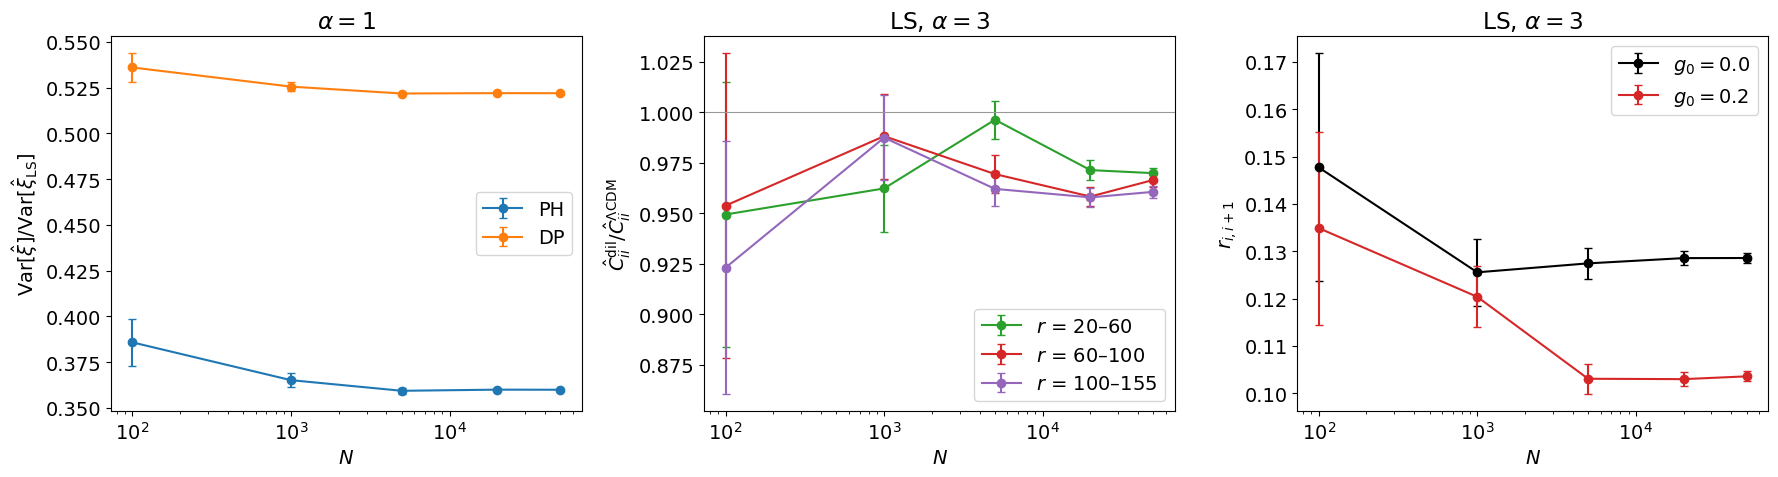
\includegraphics[width=\linewidth]{convergencia.png}
                \caption{Convergencia con $N$ de tres cantidades. A la izquierda, la varianza de Peebles--Hauser y Davis--Peebles entre la de Landy--Szalay ($\alpha = 1$); al centro, el cociente de varianzas con y sin dilución para Landy--Szalay en tres rangos de $r$ ($\alpha = 3$); a la derecha, la correlación entre \emph{bins} vecinos de Landy--Szalay. Los errores son de \emph{bootstrap}.}
                \label{fig:convergencia}
            \end{figure}

            \begin{table}[H]
                \centering
                \caption{Comparación entre las predicciones de la Sección~\ref{sec:predicciones} y lo medido con $N = 5\times10^4$.}
                \label{tab:resultados}
                \begin{tabular}{lll}
                    \toprule
                    Cantidad & Predicción & Medido \\
                    \midrule
                    ${\rm Var}_{\rm PH}/{\rm Var}_{\rm LS}$, $\alpha = 1$ & $0.33$ (Poisson) & $0.360 \pm 0.001$ \\
                    ${\rm Var}_{\rm DP}/{\rm Var}_{\rm LS}$, $\alpha = 1$ & $0.50$ (Poisson) & $0.522$ \\
                    ${\rm Var}_{\rm PH}/{\rm Var}_{\rm LS}$, $\alpha = 3$ & $0.60$ (Poisson) & $0.627 \pm 0.001$ \\
                    ${\rm Var}_{\rm DP}/{\rm Var}_{\rm LS}$, $\alpha = 3$ & $0.70$ (Poisson) & $0.721$ \\
                    ${\rm Var}_{\rm Ham}/{\rm Var}_{\rm LS}$ & $1$ & $1.01$ ($\alpha = 1$), $1.00$ ($\alpha = 3$) \\
                    ${\rm Var}_{\rm PH}/{\rm Var}_{\rm LS}$ con dilución, $\alpha = 1$ & $0.352 \pm 0.002$ ($c \to [A^2c, Ac]$) & $0.353 \pm 0.001$ \\
                    ${\rm Var}_{\rm PH}/{\rm Var}_{\rm LS}$ con dilución, $\alpha = 3$ & $0.620 \pm 0.002$ ($c \to [A^2c, Ac]$) & $0.620 \pm 0.001$ \\
                    \midrule
                    $C_{ii}^{\rm dil}/C_{ii}^{\LCDM}$, PH, $\alpha = 3$ & entre $0.64$ y $1$ & $0.953 \pm 0.002$ \\
                    $C_{ii}^{\rm dil}/C_{ii}^{\LCDM}$, DP, $\alpha = 3$ & entre $0.64$ y $1$ & $0.958 \pm 0.002$ \\
                    $C_{ii}^{\rm dil}/C_{ii}^{\LCDM}$, Ham, $\alpha = 3$ & entre $0.64$ y $1$ & $0.965 \pm 0.002$ \\
                    $C_{ii}^{\rm dil}/C_{ii}^{\LCDM}$, LS, $\alpha = 3$ & entre $0.64$ y $1$ & $0.965 \pm 0.002$ \\
                    \midrule
                    $r_{i,i+1}^{\rm dil}/r_{i,i+1}^{\LCDM}$, LS & entre $0.66$ y $0.83$ & $0.81 \pm 0.01$ \\
                    \bottomrule
                \end{tabular}
            \end{table}

        \subsection{Limitaciones}

            Es importante tener presentes las limitaciones del análisis. Todo es lineal, en espacio real y solo para la materia, así que no incluye términos no lineales, distorsiones al espacio de \emph{redshift} ni sesgo de trazadores. La transformación lognormal y el muestreo en una malla de $7.8\,\hMpc$ modifican ligeramente la función de correlación de los catálogos respecto a la ecuación \eqref{eq:xi_teo}, aunque el efecto es pequeño para $r \geq 20\,\hMpc$. La covarianza gaussiana de la ecuación \eqref{eq:cov_gauss} solo se usó para predecir cómo escalan los términos y no se comparó elemento a elemento con la covarianza muestral. Por último, todos los resultados corresponden a una sola densidad de puntos: con un $\bar n$ mayor, la varianza cósmica pesaría más y el cociente entre modelos debería acercarse a $0.64$.

    %=====================================================================%
    \section{Uso de los modelos LLM}\label{sec:llm}
    %=====================================================================%

        % PENDIENTE (autor): agregar las versiones de los modelos y los enlaces a los historiales, por ejemplo:
        % La información específica se puede encontrar en los siguientes historiales:
        % \begin{enumerate}
        %     \item \url{https://claude.ai/share/...}
        % \end{enumerate}
        A lo largo de este trabajo se utilizaron modelos de lenguaje (LLM) de Anthropic (Claude), principalmente a través de \emph{Claude Code}, para acelerar el proceso.

        % PENDIENTE: confirmar estas frases después de revisar el texto y las derivaciones.
        Este reporte en particular se escribió con ayuda de \emph{Claude Code}: a partir del \emph{notebook}, del plan del proyecto y de las diapositivas, el modelo generó la estructura y un primer borrador que después se corrigió. Las estimaciones de Poisson de la Sección~\ref{sec:predicciones} y la explicación del sesgo por el catálogo aleatorio fijo surgieron en esa misma conversación y se comprobaron contra los resultados numéricos, con los que coinciden. También se usó para escribir el código de producción en Slurm (\texttt{slurm/farm.py}), para editar la presentación y para revisar el código y el texto; de esas revisiones salieron, entre otras correcciones, que la semilla común no comparte el ruido de Poisson entre modelos y que los cocientes entre estimadores sí dependen de $g_0$.

        % PENDIENTE (autor): si se usaron instrucciones de sistema, pegarlas aquí en un PromptBlock; si no, borrar este comentario.
        % \begin{PromptBlock}
        % SYSTEM INSTRUCTIONS
        % ...
        % \end{PromptBlock}

    %=====================================================================%
    \section{Conclusiones}\label{sec:conclusiones}
    %=====================================================================%

        El resultado principal de este trabajo es que, con la densidad de puntos usada, la covarianza de los estimadores de $\xi(r)$ casi no distingue entre $\LCDM$ y el modelo de dilución: la varianza baja apenas a $0.95$--$0.97$ de la de $\LCDM$, aunque la señal baja un 20\%. La explicación está en la estructura de la covarianza gaussiana, donde solo la varianza cósmica escala como $P^2$; con $\bar n = 5\times10^{-5}\,h^3\,\mathrm{Mpc}^{-3}$ domina el ruido de Poisson, que no se diluye. Lo que sí se diluye es la parte que correlaciona \emph{bins} distintos, y por eso la correlación entre \emph{bins} vecinos baja de $0.129$ a $0.104$. En la práctica, esto significa que una covarianza calculada en $\LCDM$ serviría para poner a prueba la dilución a orden lineal.

        La comparación entre estimadores dio un resultado que va en contra de lo que normalmente se recomienda: en una caja periódica y con un catálogo aleatorio fijo, Peebles--Hauser tiene la menor varianza y Landy--Szalay y Hamilton la mayor. Esto no es un error, sino una consecuencia de que no haya bordes, ya que la ventaja de Landy--Szalay depende de ellos. Los cocientes siguen bastante bien la estimación de Poisson $2 : (2 + 1/\alpha) : (2 + 4/\alpha)$ más un término común de varianza cósmica, y dependen de la dilución solo a través de ese término, que al diluirse los baja en ${\sim}0.007$.

        El cuello de botella de todo el trabajo fue el conteo de pares. El plan original contemplaba unas 100 realizaciones por modelo, pero con ese número el error de cada varianza es de ${\sim}14\%$ y no hay forma de resolver un cambio de $4\%$. Fue necesario llevar el cálculo a Slurm y usar un nodo completo para llegar a $5\times10^4$ realizaciones, y valió la pena por dos razones: con $N = 5000$ parecía que el cociente entre modelos dependía de $r$ y resultó ser una fluctuación, y fue con $N$ grande que el sesgo del catálogo aleatorio fijo quedó claramente separado del ruido. Este sesgo es, quizás, la lección práctica más útil, porque aumentar $N$ no lo corrige y hay que atacarlo desde los catálogos aleatorios.

        Durante el desarrollo se exploraron más cosas de las que aparecen aquí, como la covarianza gaussiana analítica, el espectro de potencias medido $\hat P(k)$, varias densidades de puntos, la derivada $\partial C/\partial g_0$ y un ajuste de amplitud, pero se dejaron fuera para mantener el alcance del proyecto. Todas estas posibilidades, junto con repetir el análisis con densidades mayores, variar $g_0$, $z_t$ y $\Delta z$, usar un catálogo aleatorio distinto en cada realización o el $\RR$ analítico, estudiar geometrías con bordes y llevar el mismo análisis al espacio de Fourier, se dejan para un trabajo futuro. Por último, como a un $z$ fijo la dilución es degenerada con $\sigma_8$, distinguirla de verdad requiere el crecimiento a varios \emph{redshifts} o las velocidades, a través de la combinación $f + g$ en el espacio de \emph{redshift}.

    %=====================================================================%
    \begin{thebibliography}{99}
    %=====================================================================%

        \bibitem{desi_dr2} DESI Collaboration, Abdul-Karim, M., et al. (2025). DESI DR2 Results II: Measurements of Baryon Acoustic Oscillations and Cosmological Constraints. arXiv preprint arXiv:2503.14738. \url{https://arxiv.org/abs/2503.14738}

        \bibitem{planck2018} Planck Collaboration, Aghanim, N., et al. (2020). Planck 2018 results. VI. Cosmological parameters. \textit{Astronomy \& Astrophysics}, 641, A6. \url{https://arxiv.org/abs/1807.06209}

        \bibitem{camphuis} Camphuis, E., et al. (SPT-3G Collaboration) (2025). SPT-3G D1: CMB temperature and polarization power spectra and cosmology from 2019 and 2020 observations of the SPT-3G Main field. arXiv preprint arXiv:2506.20707. \url{https://arxiv.org/abs/2506.20707}

        \bibitem{chen_loeb} Chen, X., \& Loeb, A. (2025). Evolving Dark Energy or Evolving Dark Matter? \textit{Journal of Cosmology and Astroparticle Physics}, 2025(07), 059. \url{https://arxiv.org/abs/2505.02645}

        \bibitem{aviles_ferrara} Avilés, A., \& Ferrara, J. (en preparación). Dark Matter Dilution: A Two-Field Lagrangian Perturbation Theory of Large-Scale Structure. Borrador.

        \bibitem{khoury2025} Khoury, J., Lin, M.-X., \& Trodden, M. (2025). Apparent $w<-1$ and a Lower $S_8$ from Dark Axion and Dark Baryons Interactions. \textit{Physical Review Letters}, 135, 181001. \url{https://arxiv.org/abs/2503.16415}

        \bibitem{khoury2026} Khoury, J., Lin, M.-X., \& Trodden, M. (2026). Cosmological Evidence for Dark Axion--Dark Baryon Interactions from Apparent Phantom Crossing. arXiv preprint arXiv:2607.16191. \url{https://arxiv.org/abs/2607.16191}

        \bibitem{silva} Silva, E., Hartmann, G., \& Nunes, R. C. (2026). One-loop power spectrum corrections in interacting dark energy cosmologies. \textit{Physical Review D}, 113, 063548. \url{https://arxiv.org/abs/2512.11678}

        \bibitem{steele_smith} Steele, T., \& Smith, R. E. (2026). An efficient model of cosmology dependence in the covariance matrix of the matter power spectrum. arXiv preprint arXiv:2601.13245. \url{https://arxiv.org/abs/2601.13245}

        \bibitem{kolonia} Kolonia, E.-A., Li, H., Zhang, H., \& Afshordi, N. (2026). Stable cosmology under flexible covariances: Rescaling and cross-survey correlations in DESI BAO and supernova data. arXiv preprint arXiv:2611.13829. \url{https://arxiv.org/abs/2611.13829}

        \bibitem{mukherjee} Mukherjee, D., \& Räsänen, S. (2026). Cosmic variance and ergodicity in finite systems with correlations. arXiv preprint arXiv:2608.30838. \url{https://arxiv.org/abs/2608.30838}

        \bibitem{peebles_hauser} Peebles, P. J. E., \& Hauser, M. G. (1974). Statistical Analysis of Catalogs of Extragalactic Objects. III. The Shane-Wirtanen and Zwicky Catalogs. \textit{The Astrophysical Journal Supplement Series}, 28, 19.

        \bibitem{davis_peebles} Davis, M., \& Peebles, P. J. E. (1983). A survey of galaxy redshifts. V. The two-point position and velocity correlations. \textit{The Astrophysical Journal}, 267, 465.

        \bibitem{hamilton} Hamilton, A. J. S. (1993). Toward Better Ways to Measure the Galaxy Correlation Function. \textit{The Astrophysical Journal}, 417, 19.

        \bibitem{landy_szalay} Landy, S. D., \& Szalay, A. S. (1993). Bias and Variance of Angular Correlation Functions. \textit{The Astrophysical Journal}, 412, 64.

        \bibitem{kerscher} Kerscher, M., Szapudi, I., \& Szalay, A. S. (2000). A Comparison of Estimators for the Two-Point Correlation Function. \textit{The Astrophysical Journal Letters}, 535, L13.

        \bibitem{hartlap} Hartlap, J., Simon, P., \& Schneider, P. (2007). Why your model parameter confidences might be too optimistic. Unbiased estimation of the inverse covariance matrix. \textit{Astronomy \& Astrophysics}, 464, 399.

        \bibitem{grieb} Grieb, J. N., Sánchez, A. G., Salazar-Albornoz, S., \& Dalla Vecchia, C. (2016). Gaussian covariance matrices for anisotropic galaxy clustering measurements. \textit{Monthly Notices of the Royal Astronomical Society}, 457, 1577.

        \bibitem{wang_cov} Wang, Y., Zhao, R., Zhao, G.-B., \& Koyama, K. (2026). A Gaussian Covariance Matrix for Joint Pre- and Post-Reconstruction Full-Shape Power Spectrum Analysis. arXiv preprint arXiv:2608.05504. \url{https://arxiv.org/abs/2608.05504}

        \bibitem{numpy} Harris, C. R., et al. (2020). Array programming with NumPy. \textit{Nature}, 585, 357.

        \bibitem{scipy} Virtanen, P., et al. (2020). SciPy 1.0: Fundamental Algorithms for Scientific Computing in Python. \textit{Nature Methods}, 17, 261.

        \bibitem{class} Blas, D., Lesgourgues, J., \& Tram, T. (2011). The Cosmic Linear Anisotropy Solving System (CLASS). Part II: Approximation schemes. \textit{Journal of Cosmology and Astroparticle Physics}, 2011(07), 034. \url{https://arxiv.org/abs/1104.2933}

        \bibitem{coles_jones} Coles, P., \& Jones, B. (1991). A lognormal model for the cosmological mass distribution. \textit{Monthly Notices of the Royal Astronomical Society}, 248, 1.

    \end{thebibliography}

\end{document}
